\documentclass[11pt]{article}

\usepackage{amssymb, amsmath, amsthm}
\usepackage[arrow,matrix,curve,cmtip,ps]{xy}
\usepackage{bm}
\usepackage{verbatim}
\usepackage[toc,page]{appendix}
\usepackage[english]{babel}
\usepackage{color}
\usepackage[utf8]{inputenc}
\usepackage{fancyhdr}
\usepackage{float}
\usepackage{geometry}
\geometry{
 a4paper,
 total={170mm,257mm},
 left=20mm,
 top=30mm,
 bottom=20mm,
}
\usepackage{graphicx}
\usepackage{fancyvrb}
\usepackage{longtable}
\usepackage[section]{placeins}
\usepackage{subcaption}
\usepackage{tabularx}
\usepackage[hyphens]{url}

\setlength{\parindent}{0.0em}
\setlength{\parskip}{0.5em}
\renewcommand{\baselinestretch}{1.3}

\newcommand\Tstrut{\rule{0pt}{2.6ex}}
\newcommand\Bstrut{\rule[-0.9ex]{0pt}{0pt}}
\newcommand{\tline}{\Tstrut\Bstrut\\}

\pagestyle{fancy}
\fancyhf{}
\rhead{Daniel Woolnough z5116128}
\chead{COMP9417 - Project}
\lhead{\today}
\cfoot{\thepage}

\newcommand{\vect}[1]{\mbox{$\bm{#1}$}}
\newcommand{\ds}{\displaystyle}

%\addtolength{\topmargin}{-3\baselineskip}
%\addtolength{\textheight}{6\baselineskip}
%\addtolength{\textwidth}{2cm}
%\addtolength{\oddsidemargin}{-1cm}
%\addtolength{\evensidemargin}{-1cm}

\begin{document}

\begin{center}
\textbf{\large{COMP9417 Machine Learning Project}}
\\[10pt]
\textbf{\huge{Classification via Robust SVMs: A Comparison on the Wisconsin Breast Cancer Dataset}}
\\[10pt]
{\it \large{Daniel Woolnough, z5116128, Group h5116128, \today}}
\end{center}
\section*{Introduction}
Support Vector Machines (SVMs) are a useful machine learning tool for classification of labelled data into distinct sets, and are capable of modelling both linear and non-linear separable datasets via kernelization and projection into higher dimensional spaces. Recently, the Robust SVM (rSVM) has been proposed, which provides immunity to uncertainty in the dataset and has an easy reformulation as a second-order cone program (SOCP), a convex optimisation problem that is easily solvable by, e.g., interior-point methods. Other SVMs are the Doubly-regularized SVM (DrSVM), the Hybrid Huberised SVM (HHSVM) and the $pg$-SVM. 

The aim of this report is to assess some of these SVMs, and some other classification techniques (including a decision tree, a naive Bayes approach, and a neural network) on a well-used dataset, the Wisconsin Breast Cancer dataset (available here: \url{https://www.kaggle.com/uciml/breast-cancer-wisconsin-data}). In particular, we wish to evaluate the rSVM in the case where the given training set is noisy/uncertain, and classifications need to be made taking this into account. 

This report is broken up into four sections:
\begin{enumerate}
	\item We describe the dataset and the preprocessing carried out on it, to prepare it for use. 
	\item We compare a Decision Tree, a Gaussian Naive Bayes classifier, a Two-Layered Perceptron (Neural Network), and a standard SVM by their performance on the (preprocessed) dataset. 
	\item We define the mathematical formulations of the classic SVM, the DrSVM, and the rSVM, that are used to implement the methods in MATLAB. MATLAB has been chosen for its more powerful optimisation toolkits and its more user-friendly interface. 
	\item Finally, we evaluate these three SVMs on the dataset, now affected by noise. 
\end{enumerate}

The selected metric over which we evaluate models is simply the raw accuracy of the model on the dataset, as expected on the Kaggle webpage.

\section{The Wisconsin Breast Cancer Dataset, and Preprocessing}

The dataset contains 569 items and 32 columns:
\begin{itemize}
	\item The first column is the item ID, numbered from 0 through 568. 
	\item The second column is the target, which is the diagnosis of the cancer as malignant (M) or benign (B). There are 357 benign diagnoses, and 212 malignant diagnoses, giving a class distribution of $[0.63, 0.37]$. 
	\item The remaining thirty columns contain the mean, standard error, and extremal value (worst-case measurement) of 10 features: radius, texture, perimeter, area, smoothness, compactness, concavity, concave points, symmetry, and fractal dimension. 
\end{itemize}
For this dataset the following preprocessing was done:
\begin{itemize}
	\item The ID column was dropped, as it does not affect the diagnosis. 
	\item The diagnoses were mapped to the numeric values: 0 if benign, 1 if malignant. 
	\item It was revealed there were no missing or NaN values in the dataset. 
	\item Each column was normalised, by recentering at 0 (subtracting the mean), and dividing through byb the standard deviation. 
	\item Finally, columns that had a correlation coefficient $< 0.1$ with the target value were dropped, as these were decided to be uncorrelated with the target, and therefore would not affect the diagnosis. 
\end{itemize}
The correlation of each feature with the diagnosis (ordered as in the dataset, so diagnosis at position 0, etc.) is shown below. 

\begin{figure}[htb!]
	\centering
	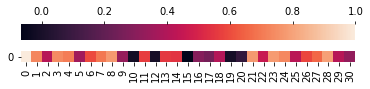
\includegraphics[width=0.75\textwidth]{corr}
\end{figure}

This process is carried out by \texttt{preprocessing.py}, which then saves the resulting dataset in a new csv file. The corresponding notebook also demonstrates this process step by step. 

\section{Comparison of Non-Robust Methods}

Taking our preprocessed dataset, we wish to make some preliminary comparisons of some common methods, to motivate the rest of the report. We chose the following (non-robust) methods:
\begin{itemize}
	\item A decision tree, with the minimum number of samples at each leaf set to 2\% of the training set, to avoid overfitting. It was determined that anything less than 1\% would overfit, while anything over 4\% would underfit. 
	\item A Gaussian Naive Bayes classifier. A Gaussian model was chosen since our data was previously normalised. To accommodate the Bayesian assumption of independence of features (which clearly doesn't hold between, for example, radius mean, standard error, and extremal value), this classifier only considered the extremal values of each core feature. 
	\item A Two-Layered Perceptron (neural network). The hidden layer was chosen to be twice the size of the input dimension (i.e. twice the number of features), with tanh activation at the hidden layer, and sigmoid activation at the output. The model was trained via stochastic gradient descent, and an adaptive learning rate initialised at 0.1. 
	\item A Support Vector Machine, with a linear kernel function and regularisation parameter set to 0.05. The regularisation parameter was determined through a grid search which showed the optimal choice to mostly lie in the range $[0, 0.1]$. 
\end{itemize}
For 100 simulations, a model was created and then trained on 80\% of the dataset, and tested on the remaining 20\%. For each simulation the accuracy (proportion of predictions which were correct) were recorded, as was the average of all simulations; see Table 1. We also recorded the F1 score for each model, for each simulation, to assess the reliability of the accuracy given the slight class imbalance; see Table 2. 

\begin{table}[H]
	\centering
	\captionsetup{font=footnotesize}
	\begin{tabular}{| c || c | c | c | c | c || c |}
		\hline
		\textbf{Model} & \textbf{Sim.	1} & \textbf{Sim. 2} & \textbf{Sim. 3} & \textbf{Sim. 4} & \textbf{Sim. 5} & \textbf{Average} 
		\tline\hline
		Decision Tree & 0.9211 & 0.9386 & 0.9474 & 0.9298 & 0.9561  & 0.9326 
		\tline\hline
		Gaussian NB & 0.9737 & 0.9474 & 0.9298 & 0.9474 & 0.9474 & 0.9445
		\tline\hline
		Neural Network & 0.9912 & 0.9825 & 1.0000 & 0.9386 & 0.9474 & 0.9729
		\tline\hline
		Support Vector Machine & 0.9912 & 0.9825 & 0.9912 & 0.9649 & 0.9737 & 0.9736
		\tline\hline
	\end{tabular}
	\caption{Accuracy results for the four basic models. Sim $i$ is the accuracy for the $i^{\rm th}$ simulation; Average is the average accuracy over 100 simulations.}
\end{table}

\begin{table}[H]
	\centering
	\captionsetup{font=footnotesize}
	\begin{tabular}{| c || c | c | c | c | c || c |}
		\hline
		\textbf{Model} & \textbf{Sim.	1} & \textbf{Sim. 2} & \textbf{Sim. 3} & \textbf{Sim. 4} & \textbf{Sim. 5} & \textbf{Average} 
		\tline\hline
		Decision Tree & 0.9072 & 0.9213 & 0.9211 & 0.8974 & 0.9398 & 0.9082
		\tline\hline
		Gaussian NB & 0.9684 & 0.9348 & 0.9070 & 0.9231 & 0.9250 & 0.9252
		\tline\hline
		Neural Network & 0.9897 & 0.9738 & 1.0000 & 0.9091 & 0.9231 & 0.9633
		\tline\hline
		Support Vector Machine & 0.9897 & 0.9783 & 0.9877 & 0.9487 & 0.9620 & 0.9638
		\tline\hline
	\end{tabular}
	\caption{F1 scores for the four basic models. Sim $i$ is the F1 score for the $i^{\rm th}$ simulation; Average is the average F1 score over 100 simulations.}
\end{table}
From the results we can see that, on average, the tuned SVM just outperforms the tuned Neural Network with one hidden layer, and is the best performing model of the four. We can also see the accuracies are reliable in that their deviation from the F1 score is small. Therefore, it is worth considering SVMs more generally in the rest of the report; in the following sections we will define four different SVM models and their mathematical formulations, and then compare their performance in a noisy setting. 

\section{Different SVM Models}

We now present the four different SVM models that we will compare in the next section: the standard SVM, the DrSVM, the $pq$-SVM, and the robust SVM. Each of these have been implemented from scratch in MATLAB, with the use of the optimisation package MOSEK, interfaced through YALMIP. The corresponding MATLAB live script gives a simple example demonstrating the implementation and solution retrieval for each.

We denote the number of datapoints as $m$, and the number of features as $n$. 

\subsection{Standard SVM}

For this report, we take the standard SVM model as described in the lectures to be that with soft margins, as we do not want to assume linear separability. The primal formulation for this problem is
\begin{eqnarray*}
& \ds \min_{\pmb{w}\in\mathbb{R}^m,\gamma,\pmb{\xi}\in\mathbb{R}^n} & \frac{1}{2}\Vert \bm{w} \Vert_2^2  + \lambda\bm{e}^T\bm{\xi} 
\\
& \mbox{ subject to } & Y(X\bm{w} - \bm{e}\gamma) + \bm{\xi} \geq \bm{e} 
\\
& & \bm{\xi} \geq 0
\end{eqnarray*}
where $\bm{x}_i\in\mathbb{R}^n$ is the $i^{\rm th}$ data point, $X\in\mathbb{R}^{m\times n}$ is a matrix whose $i^{\rm th}$ row is $\bm{x}_i$, $\bm{y}\in\mathbb{R}^m$ is the classification vector (with each element $y_i$ in $\{-1, 1\}$), $Y = {\rm diag}(\bm{y})\in\mathbb{R}^{m\times m}$, and $\bm{e} = (1, 1, \dots, 1)^T\in\mathbb{R}^{m}$. The optimisation variables are $\bm{w}$, the weight vector, $\gamma$ the bias, and $\bm{\xi}$, the misclassification error for $X$: that is, $\xi_i = 0$ if ${\rm sign}(\bm{w}^T\bm{x}_i - \gamma) = y_i$, otherwise $\xi_i > 0$, $i=1,\dots,m$. 

Typically we solve $(SVM)$ by instead formulating and solving the dual problem, as this (a) allows for us to more efficiently the solve the problem if we wish to apply the kernel trick for high-dimensional embedding, and (b) still be able to retrieve the values for $\bm{w}$ and $\gamma$. The dual problem is given by
\begin{eqnarray*}
(SVM) & \ds\min_{\pmb{u}\in\mathbb{R}^m} & \frac{1}{2} \bm{u}YXX^TY^T\bm{u} - \bm{e}^T\bm{u}
\\
& \mbox{subject to } & \bm{e}^TY^T\bm{u} = 0
\\
& & 0 \leq \bm{u} \leq \nu\bm{e}
\end{eqnarray*}
The original solution is then retrieved as follows: $\bm{x}_j$ is a support vector iff $u_j\neq 0$, $j=1,\dots,m$; $\bm{w} = X^TY^T\bm{u}$; and $\gamma$ satisfies $y_j(\bm{w}^T\bm{x}_j - \gamma) = 1$ for support vector $\bm{x}_j$. 

\subsection{DrSVM \cite{drsvm}}

\subsection{$pq$-SVM \cite{pqsvm}}

\subsection{Robust SVM \cite{rsvm}}

\begin{thebibliography}{99}

\bibitem{drsvm} L. Wang, J. Zhu, and H. Zou: ``The Doubly Regularized Support Vector Machine'', \emph{Statistica Sinica}, (16), 589–615, 2006.

\bibitem{pqsvm} M. Dunbar, J. Murray, L. Cysique, B. Brew, V. Jeyakumar: ``Simultaneous classification and feature selection via convex quadratic programming with application to HIV-associated neurocognitive disorder assessment'', \emph{European Journal of Operational Research}, (206)2, 470–478, 2010.

\bibitem{rsvm} M. A. Goberna, V. Jeyakumar, G. Li: ``Calculating Radius of Robust Feasibility of Uncertain Linear Conic Programs via Semidefinite Programs'', \emph{UNSW Preprint}, \url{https://arxiv.org/abs/2007.07599}, 2020.


\end{thebibliography}

\end{document}